\section{Egyéb követelmények}
\newcounter{Ecounter}
\newcommand{\sorSzamE}{\stepcounter{Ecounter}\theEcounter}

A \textit{Segítség, építkezem!} weboldal első körben magyar nyelven kell készüljön (\kovAzon{E\_\sorSzamE}). Az oldal minden képernyőméretben jól használható (\kovAzon{E\_\sorSzamE}) és akadálymentesített kell legyen, illetve rendelkeznie kell nagy kontrasztú változattal (\kovAzon{E\_\sorSzamE}).

\section{Felhasználói esetdiagram}

A \ref{fig:use_case}. ábra bemutatja az egyes szerepkörökkel rendelkező felhasználók lehetséges tevékenységeit az oldalon.

\begin{figure}[h]
	\centering
	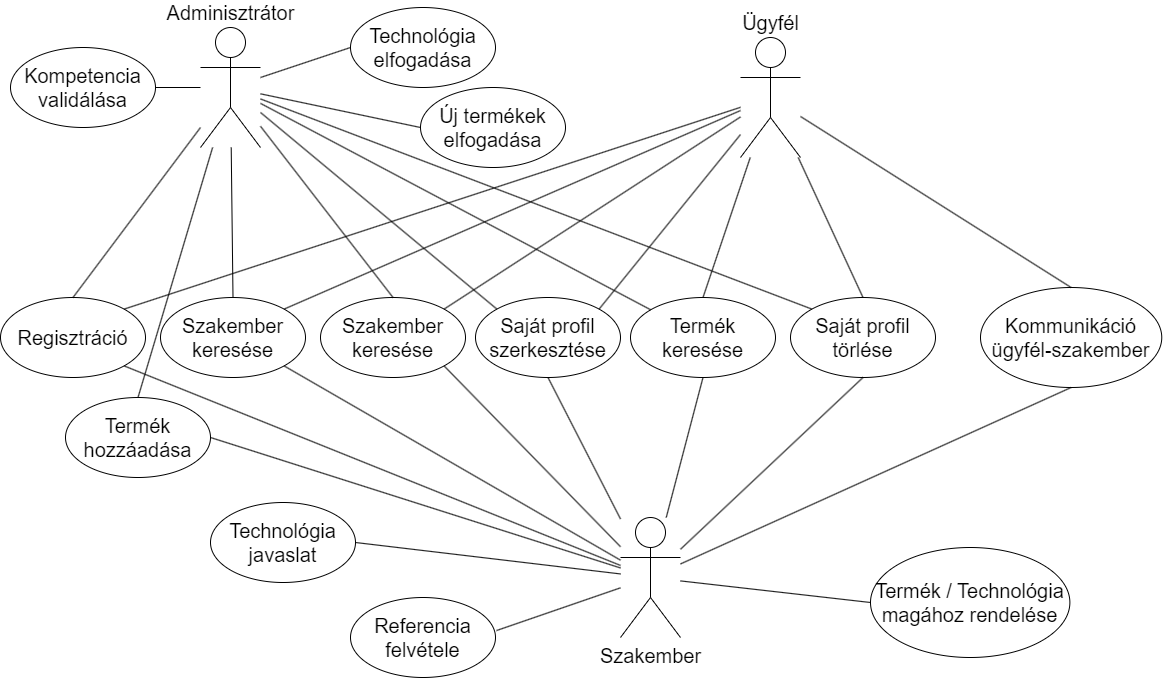
\includegraphics[scale=0.3]{img/Use_Case_Diagram.png}
	\caption{Felhasználói esetdiagram}
	\label{fig:use_case}
\end{figure}